\subsection{Overview}

How to solve the problem of similarity between documents, subsection about SVD, LSI and other techniques.

\subsection{Mathematical Background}

%%%%%%%%%%%%%%%%%%%%%%%%%%%%%%%%%%%%%%%%%%%%%%%%%%%%%%%%%%

\subsubsection{Term-Document Matrix}
 In Natural Language Processing \cite{Collobert:2011:NLP:1953048.2078186}, a term-document matrix (TDM) is used to represent the relationships between words and documents \cite{Turney:2010:FMV:1861751.1861756}. In a TDM, each row corresponds to a document and each column corresponds to a term. A cell in the TDM represents the weight of a term in a document. The most common weighting scheme used in document retrieval is the \emph{term frequency-inverse document frequency (tf-idf)} function \cite{Reed:2006:TNT:1193211.1193734}. If we consider a set of $n$ documents $D=(d_{1},d_{2},..,d_{n})$ and a set of terms $t=(t_{1},t_{2},..,t_{r})$ then the representation of a document $d \in D $ is vector $\vec{\delta}=(w_{1}^{d},w_{2}^{d},..,w_{r}^{d})$, where the weight $w_{k}^{d}$ of term $k$ in document $d$ is computed using the {\em tf-idf} function \cite{Ramos1999}:

\begin{equation} \label{tfidf} %\nonumber 
w_{k}^{d} =tf\cdot idf(k,d,D)= f_{k}^{d}\cdot log\frac{n}{\left | \left \{ d\in D: t_{k} \in d \right \} \right |} 
\end{equation}

where $f_{k}^{d}$ is the frequency of term $t_{k}$ in document $d$.

Another common weighting scheme uses only the frequency of terms in documents for cells in TDM, i.e. the number of occurrence of a term in a document, instead of {\em tf-idf}. As an example, we consider a set of three simple documents $D=(d_{1},d_{2},d_{3})$ as follows:

\begin{itemize}
	\item[+] $d_{1}$: \emph{She is nice.}
	\item[+] $d_{2}$: \emph{Today is nice.}
	\item[+] $d_{3}$: \emph{Nice is a nice city.}
\end{itemize}

\begin{figure}[h!]
	\begin{equation} \nonumber
	\bordermatrix{~ & she & is & today & a & nice & city \cr	
		d_{1} 		& 1 & 1 & 0 & 0 & 1 & 0 \cr 
		d_{2} 		& 0 & 1 & 1 & 0 & 1 & 0 \cr  
		d_{3} 		& 0 & 1 & 0 & 1 & 2 & 1 \cr }
	\end{equation}
	\caption{An example of a term-document matrix}
	\label{fig:TDM}
\end{figure}

The set of terms $t$ consists of $6$ elements, i.e. $t=(she$, $is$, $today$, $a$, $nice$, $city)$ and the corresponding term-document matrix for $D$ is depicted in Figure \ref{fig:TDM}.

TDM has been exploited to characterize software systems and finally to compute similarities between them \cite{10.1109/APSEC.2004.69},\cite{10.1109ICPC.2016.7503721},\cite{McMillan:2012:DSS:2337223.2337267}. In a TDM for software systems, each row represents a package, an API call or a function and each column represents a software system. A cell in the matrix is the number of occurrence of a package/an API/function in each corresponding software system. A TDM for software systems has a similar form to the matrix shown in Figure \ref{fig:TDM} where documents are replaced by software systems and terms are replaced by API calls.

%%%%%%%%%%%%%%%%%%%%%%%%%%%%%%%%%%%%%%%%%%%%%%%%%%%%%%%%%%

\subsubsection{Cosine Similarity}

Cosine similarity is a metric used to compute similarity between two objects using their feature vectors \cite{tversky1977features}. An object is characterized as a vector, and for a pair of vectors $\vec{\alpha}=(\alpha_{1},\alpha_{2},..,\alpha_{n})$ and $\vec{\beta}=(\beta_{1},\beta_{2},..,\beta_{n})$ there is an angle between them. Intuitively, the cosine similarity metric measures the similarity as the cosine of the corresponding angle between the two vectors and it is computed using the inner product as follows. 

\begin{equation} \label{eqn:Cosine}
CosineSim(\vec{\alpha},\vec{\beta}) = \frac{\sum_{i=1}^{n}\alpha_{i}\cdot \beta_{i}}{\sqrt{\sum_{i=1}^{n}(\alpha_{i})^{2} }\cdot \sqrt{\sum_{i=1}^{n}(\beta_{i})^{2}}}
\end{equation}

Figure \ref{fig:Cosine} illustrates the cosine similarity between two vectors $\vec{\alpha}$ and $\vec{\beta}$ in a three-dimension space. This can be thought as the similarity between two documents with three terms $t=(t_{1},t_{2},t_{3})$.

\begin{figure}[h!]
	\centering
	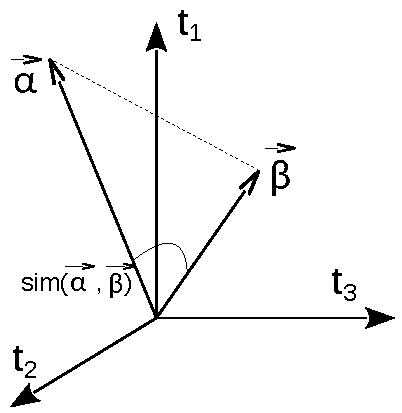
\includegraphics[width=0.25\textwidth]{images/Cosine.pdf}
	\caption{Cosine similarity between two feature vectors $\vec{\alpha}$ and $\vec{\beta}$}
	\label{fig:Cosine}
\end{figure}

Cosine similarity has been popularly adopted in many applications that are related to similarity measurement in various domains \cite{Huang:2012:LCD:2343876.2343884},\cite{Islam:2008:STS:1376815.1376819},\cite{Linden:2003:ARI:642462.642471},\cite{conf:iscis:MadylovaO09},\cite{Mihalcea:2006:CKM:1597538.1597662}. Among the similarity metrics being recalled in this deliverable, the prevalence of Cosine Similarity is obvious as it is utilized in almost all of them as follows: \textit{MUDABlue} \cite{10.1109/APSEC.2004.69}, \textit{CLAN} \cite{McMillan:2012:DSS:2337223.2337267}, \textit{CLANdroid} \cite{10.1109ICPC.2016.7503721}, \textit{LibRec} \cite{6671293}, \textit{SimApp} \cite{Chen:2015:SFD:2684822.2685305}, \textit{WuKong} \cite{Wang:2015:WSA:2771783.2771795}, \textit{TagSim} \cite{Lo:2012:DSA:2473496.2473616}, and \textit{RepoPal} \cite{10.1109/SANER.2017.7884605}

%%%%%%%%%%%%%%%%%%%%%%%%%%%%%%%%%%%%%%%%%%%%%%%%%%%%%%%%%%  

\subsubsection{Singular Value Decomposition}

\subsubsection{Latent Semantic Analysis}